\begin{tikzpicture}[remember picture, scale=\modDGHyperScale]
% dummy
\coordinate[overlay] (\modIdPrefix v-coord-0-0) at (6.5671, 1.7917) {};
\coordinate[overlay] (\modIdPrefix v-coord-1-0) at (6.8443, 6.7559) {};
\coordinate[overlay] (\modIdPrefix v-coord-2-0) at (0.7022, 3.7229) {};
\coordinate[overlay] (\modIdPrefix v-coord-3-0) at (6.0219, 3.9706) {};
\coordinate[overlay] (\modIdPrefix v-coord-4-0) at (3.4686, 1.1982) {};
\coordinate[overlay] (\modIdPrefix v-coord-5-0) at (3.2184, 6.5176) {};
\coordinate[overlay] (\modIdPrefix v-coord-6-0) at (3.3632, 3.8588) {};

% id = 0, graphName = H2O
\node[modStyleDGHyperVertex, at=(v-coord-0-0)] (v-0-0) {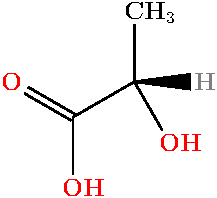
\includegraphics[scale=\modDGHyperImageScale] {\modInputPrefix/out/002_g_0_11311100.pdf}\\{$\mathrm{H2O}$}};
% id = 1, graphName = ATP
\node[modStyleDGHyperVertex, at=(v-coord-1-0)] (v-1-0) {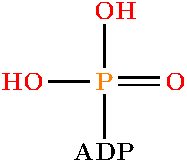
\includegraphics[scale=\modDGHyperImageScale] {\modInputPrefix/out/004_g_1_11311100.pdf}\\{$\mathrm{ATP}$}};
% id = 2, graphName = Phosphate
\node[modStyleDGHyperVertex, at=(v-coord-2-0)] (v-2-0) {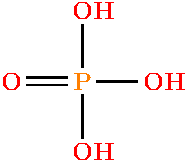
\includegraphics[scale=\modDGHyperImageScale] {\modInputPrefix/out/006_g_2_11311100.pdf}\\{$\mathrm{Phosphate}$}};
% id = 3, graphName = Cellobiose
\node[modStyleDGHyperVertex, at=(v-coord-3-0)] (v-3-0) {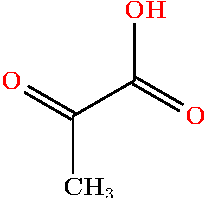
\includegraphics[scale=\modDGHyperImageScale] {\modInputPrefix/out/008_g_3_11311100.pdf}\\{$\mathrm{Cellobiose}$}};
% id = 4, graphName = p_{1,0}
\node[modStyleDGHyperVertex, at=(v-coord-4-0)] (v-4-0) {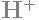
\includegraphics[scale=\modDGHyperImageScale] {\modInputPrefix/out/010_g_4_11311100.pdf}\\{$\mathrm{p_{1,0}}$}};
% id = 5, graphName = p_{1,1}
\node[modStyleDGHyperVertex, at=(v-coord-5-0)] (v-5-0) {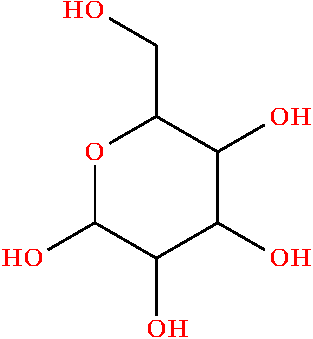
\includegraphics[scale=\modDGHyperImageScale] {\modInputPrefix/out/012_g_5_11311100.pdf}\\{$\mathrm{p_{1,1}}$}};
% id = 6{ 'Phosphate' 'Cellobiose' }, ' cellobiose + phosphate = alpha-D-glucose 1-phosphate + D-glucose', { 'p_{1,0}' 'p_{1,1}' }
\node[modStyleDGHyperEdge, at=(v-coord-6-0)] (v-6-0) {$\mathrm{r_{0}}$};
% id = 6{ 'Phosphate' 'Cellobiose' }, ' cellobiose + phosphate = alpha-D-glucose 1-phosphate + D-glucose', { 'p_{1,0}' 'p_{1,1}' }
\path[modStyleDGHyperConnector] (v-2-0) to (v-6-0);
\path[modStyleDGHyperConnector] (v-3-0) to (v-6-0);
\path[modStyleDGHyperConnector] (v-6-0) to (v-4-0);
\path[modStyleDGHyperConnector] (v-6-0) to (v-5-0);
\end{tikzpicture}%
